\documentclass[11pt]{article}
\usepackage[margin=1in]{geometry}
\usepackage{amsmath,amssymb}
\usepackage{siunitx}
\usepackage{graphicx}
\usepackage[hidelinks]{hyperref}
\usepackage{enumitem}
\graphicspath{{figures/}}

\title{\texttt{PTCryspMC.jl} --- The simulation engine\\[2pt]
\large Physics, geometry, transport, and detector response}
\author{}
\date{}

\begin{document}
\maketitle
\begin{abstract}
\noindent
\texttt{PTCryspMC.jl} is a fast, photon-only Monte Carlo that computes how a PET scanner responds
to positron annihilations. This document describes the \emph{engine}: the photon physics, the
geometry, the transport, and the detector model. The engine takes one annihilation --- a point and
two \SI{511}{keV} photons --- and returns where each photon interacts in the crystal ring, with what
energy, and at what time. The same engine drives both application modes (a geometric phantom or a
proton-beam scenario), which are described in the companion document \texttt{PTCryspMC\_app}.
\end{abstract}

\tableofcontents

\section{Introduction}

A positron emitted in tissue slows to rest and annihilates with an electron, producing two
\SI{511}{keV} photons that leave back-to-back. A PET scanner surrounds the patient with a ring of
scintillating crystal and records \emph{coincidences}: pairs of photons that arrive within a short
time window. Each coincidence defines a \emph{line of response} (LOR), the line joining the two
interaction points, along which the annihilation lay. The list of LORs is the measurement from
which an image --- and, here, the proton range --- is reconstructed.

The engine reproduces this response photon by photon. It follows only the photons: the electrons
they free travel less than a millimetre at \SI{511}{keV} and deposit their energy where they are
made, and the scintillation light is summarised by a resolution model rather than tracked
quantum by quantum. These choices keep the engine fast enough to run the order of $10^{8}$
annihilations a clinical measurement contains, for each candidate scanner.

The engine is organised in layers, each a small module: the photon physics (\S\ref{sec:physics}),
the geometry (\S\ref{sec:geometry}), the transport that moves a photon through that geometry
(\S\ref{sec:transport}), and the detector model that turns a true interaction into a measurement
(\S\ref{sec:detector}).

\section{Photon physics}
\label{sec:physics}

\subsection{The annihilation pair}

In the centre-of-mass frame the two annihilation photons leave exactly back-to-back at
\SI{511}{keV} each. The positron and electron retain a small residual momentum, so in the
laboratory the two photons depart from collinearity by a small \emph{acollinearity} angle, about
$0.5^{\circ}$ FWHM in water.

The engine models this directly. The first photon is emitted in an isotropic direction
$\mathbf{d}_1$. The second leaves along $-\mathbf{d}_1$, tilted by a two-dimensional Gaussian
deviation in the plane transverse to it: each transverse component is drawn from
$\mathcal{N}(0,\sigma)$, so each projected angle has the prescribed FWHM,
\begin{equation}
  \sigma = \frac{\theta_{\mathrm{FWHM}}}{2\sqrt{2\ln 2}}.
\end{equation}
As $\sigma\!\to\!0$ the pair is exactly antiparallel.

\subsection{Interactions: free path and process}

A photon travels in straight lines between interactions. The distance to the next interaction is
exponentially distributed with the material's total macroscopic cross section $\Sigma$
[\si{cm^{-1}}],
\begin{equation}
  p(s)\,\mathrm{d}s = \Sigma\, e^{-\Sigma s}\,\mathrm{d}s,
  \qquad s = -\frac{\ln u}{\Sigma}, \quad u\sim\mathcal{U}(0,1),
\end{equation}
and the mean free path is $1/\Sigma$. At the interaction point the process is chosen in proportion
to the partial cross sections. Two processes matter at \SI{511}{keV}:
\begin{description}[style=nextline,leftmargin=1.5em]
\item[Compton scattering.] The photon transfers part of its energy to an atomic electron and
continues at a reduced energy $E'$ in a new direction, both drawn from the Klein--Nishina
distribution (sampled by the Butcher--Messel composition--rejection method). With
$\varepsilon = E'/E$ the Compton relation gives the scattering angle,
\begin{equation}
  1 - \cos\theta = \frac{m_e c^2}{E}\,\frac{1-\varepsilon}{\varepsilon}.
\end{equation}
The electron recoil energy $E - E'$ is deposited at the interaction point.
\item[Photoelectric absorption.] The photon is absorbed and its full energy deposited at the
interaction point.
\end{description}
Pair production has a threshold of $2 m_e c^2 = \SI{1.022}{MeV}$; since these photons start at
\SI{511}{keV} and only lose energy by Compton scattering, that channel never opens.

\subsection{Cross sections}

The partial and total cross sections come from the NIST XCOM tables, tabulated per material as the
mass attenuation $\mu/\rho$ [\si{cm^2/g}]. The macroscopic cross section is the product with the
material density,
\begin{equation}
  \Sigma_{\mathrm{proc}}(E) = \Big(\tfrac{\mu}{\rho}\Big)_{\!\mathrm{proc}}(E)\,\rho ,
\end{equation}
interpolated log--log in energy. Figure~\ref{fig:xsections} shows the two materials the engine
uses most. In water at \SI{511}{keV} the cross section is almost entirely Compton: a photon born in
the patient is far more likely to scatter than to be absorbed, and that scattering is the origin of
the patient-scatter background. In the crystal the photoelectric cross section is much larger
(high-$Z$ iodine and caesium), so a crystal both Compton-scatters and fully absorbs the \SI{511}{keV}
photons --- the latter giving the full-energy photopeak the energy selection relies on.

\begin{figure}[t]
  \centering
  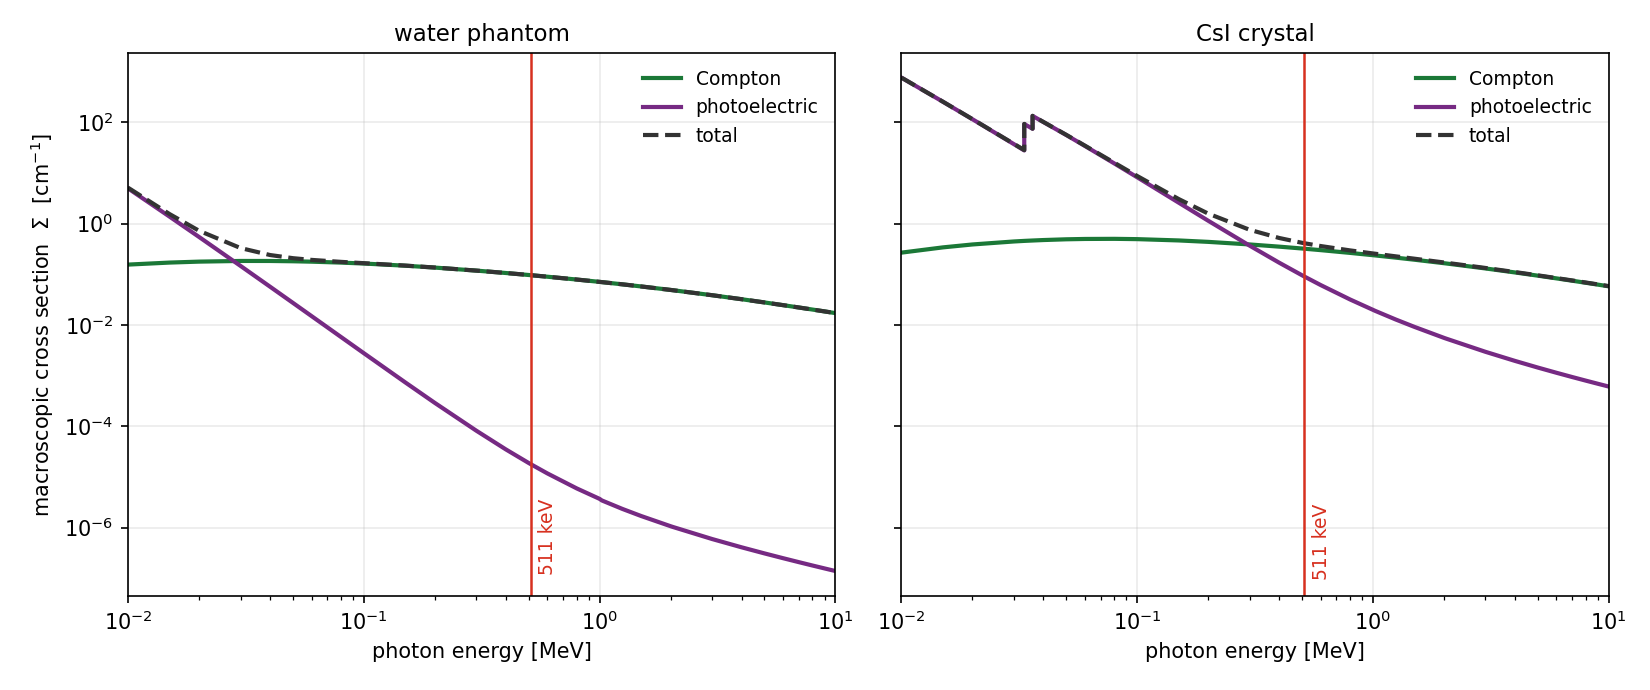
\includegraphics[width=\textwidth]{xsections}
  \caption{Macroscopic cross sections $\Sigma = (\mu/\rho)\,\rho$ for water and CsI, from the NIST
  XCOM tables. The vertical line marks \SI{511}{keV}. In water Compton dominates; in CsI the
  photoelectric cross section (with the iodine K-edge visible near \SI{33}{keV}) is comparable to
  Compton at \SI{511}{keV}.}
  \label{fig:xsections}
\end{figure}

\section{Geometry}
\label{sec:geometry}

\subsection{The volume hierarchy}

The geometry follows a Geant4-style hierarchy. A \emph{solid} is a shape in its own local frame
(cylinder, box, sphere, or cylindrical shell) that answers three questions for a ray: is a point
inside, how far to the entry surface, and how far to the exit surface --- each in closed form. A
\emph{logical volume} pairs a solid with a material; a \emph{physical volume} places a logical
volume at a position in the world. The world is itself a physical volume (a large air cylinder)
that contains the phantom and the detector ring.

\subsection{The crystal ring as a structured block/wheel grid}

The detector ring is a cylindrical shell of crystal (Fig.~\ref{fig:geometry}a). Its readout is
segmented into a structured grid: $n_\varphi$ azimuthal \emph{blocks} around the ring and $n_z$
axial \emph{wheels} along it (Fig.~\ref{fig:geometry}b). A block is one $(\varphi, z)$ cell spanning
the full radial wall depth; that radial depth is the depth-of-interaction (DOI).

Because the grid is regular, the block containing an interaction follows from arithmetic,
\begin{equation}
  i_\varphi = \Big\lfloor \frac{n_\varphi\,\varphi}{2\pi} \Big\rfloor, \qquad
  i_z = \Big\lfloor \frac{n_z\,(z + H)}{2H} \Big\rfloor,
\end{equation}
with $H$ the half-length, and the distance to the next block boundary is closed-form. The cost of
locating an interaction is therefore independent of the number of blocks --- a ring with thousands
of blocks is no more expensive to navigate than one with a handful.

\begin{figure}[t]
  \centering
  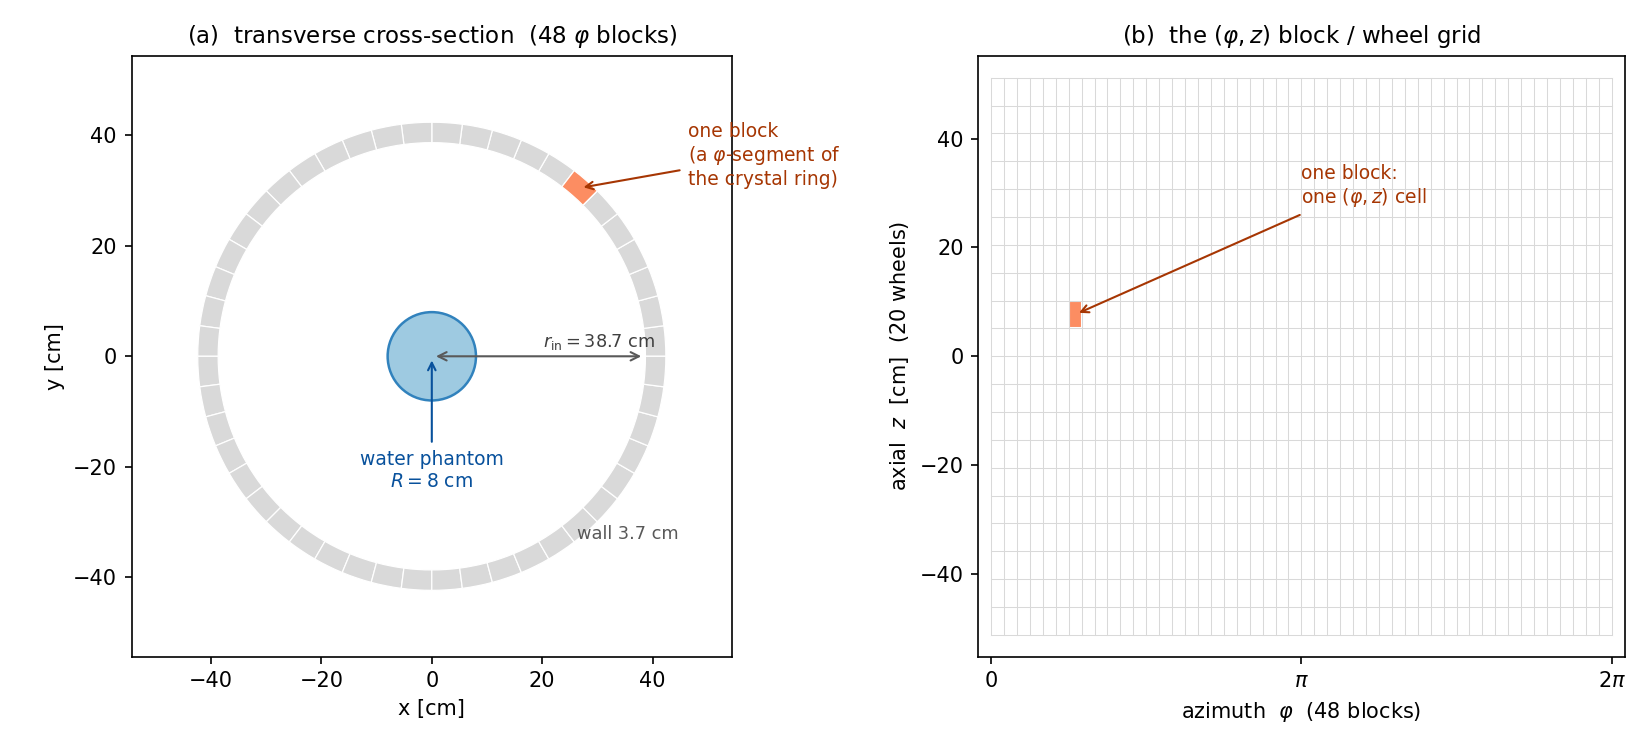
\includegraphics[width=\textwidth]{geometry}
  \caption{The scanner geometry, to scale from the run configuration. (a) Transverse cross-section:
  the water phantom ($R=\SI{8}{cm}$) at the centre of the crystal ring ($r_{\mathrm{in}}=\SI{38.7}{cm}$,
  \SI{3.7}{cm} wall), segmented into $n_\varphi = 48$ azimuthal blocks. (b) The same segmentation
  unrolled into the $(\varphi, z)$ block/wheel grid ($48 \times 20$ cells).}
  \label{fig:geometry}
\end{figure}

\section{Transport and navigation}
\label{sec:transport}

\subsection{Stepping through one volume}

Within a single volume the engine alternates sampling and moving. From the current photon state it
samples a free path; if the path reaches the volume boundary first, the photon is advanced to the
boundary; otherwise it is advanced to the interaction point, the process is chosen, the deposited
energy is recorded, and the photon either continues (Compton) with its new energy and direction or
stops (photoelectric absorption, or its energy falling below a tracking cutoff).

\subsection{Crossing volumes}

A photon born in the phantom must reach the ring through the volumes between. The navigator follows
it across boundaries, switching the material --- and therefore $\Sigma$ --- at each crossing: a
photon leaves the water phantom (where it may Compton-scatter, contributing patient scatter),
crosses the air gap, and enters the crystal. Energy is conserved across the whole path: every
recoil is deposited where it occurs, and the residual energy of an absorbed photon is accounted at
the absorption point.

\subsection{Hits: the first-interaction point}

Inside the crystal the engine forms a \emph{hit} from the deposits in a block. The hit position is
the \emph{first} interaction point, not the energy-weighted centroid: the first point is where the
photon's line of flight meets the crystal, and it is the LOR point a reconstruction aims to recover.
The hit energy is the sum of the deposits in that block, and the hit time is the earliest. A photon
that deposits in more than one block has \emph{overspilled}; a clean hit is \emph{contained} in a
single block.

Figure~\ref{fig:lor} shows what this means for a coincidence. When neither photon scatters in the
phantom, the two first-interaction points and the annihilation are collinear, and the LOR passes
through the annihilation --- a \emph{true} coincidence. When a photon Compton-scatters in the
phantom, its direction changes before it reaches the ring, so the LOR between the two hits no longer
points at the annihilation --- a \emph{scatter} coincidence, which mispositions the event. The
engine carries a per-photon phantom-scatter \emph{count} (the number of Compton interactions each
photon made in the phantom), so a coincidence can be told apart not only as true or scatter but,
among the scatters, as single ($\texttt{nscat1}+\texttt{nscat2}=1$) or multiple ($\geq 2$) --- the distinction a
scatter correction such as single-scatter simulation needs downstream.

\begin{figure}[t]
  \centering
  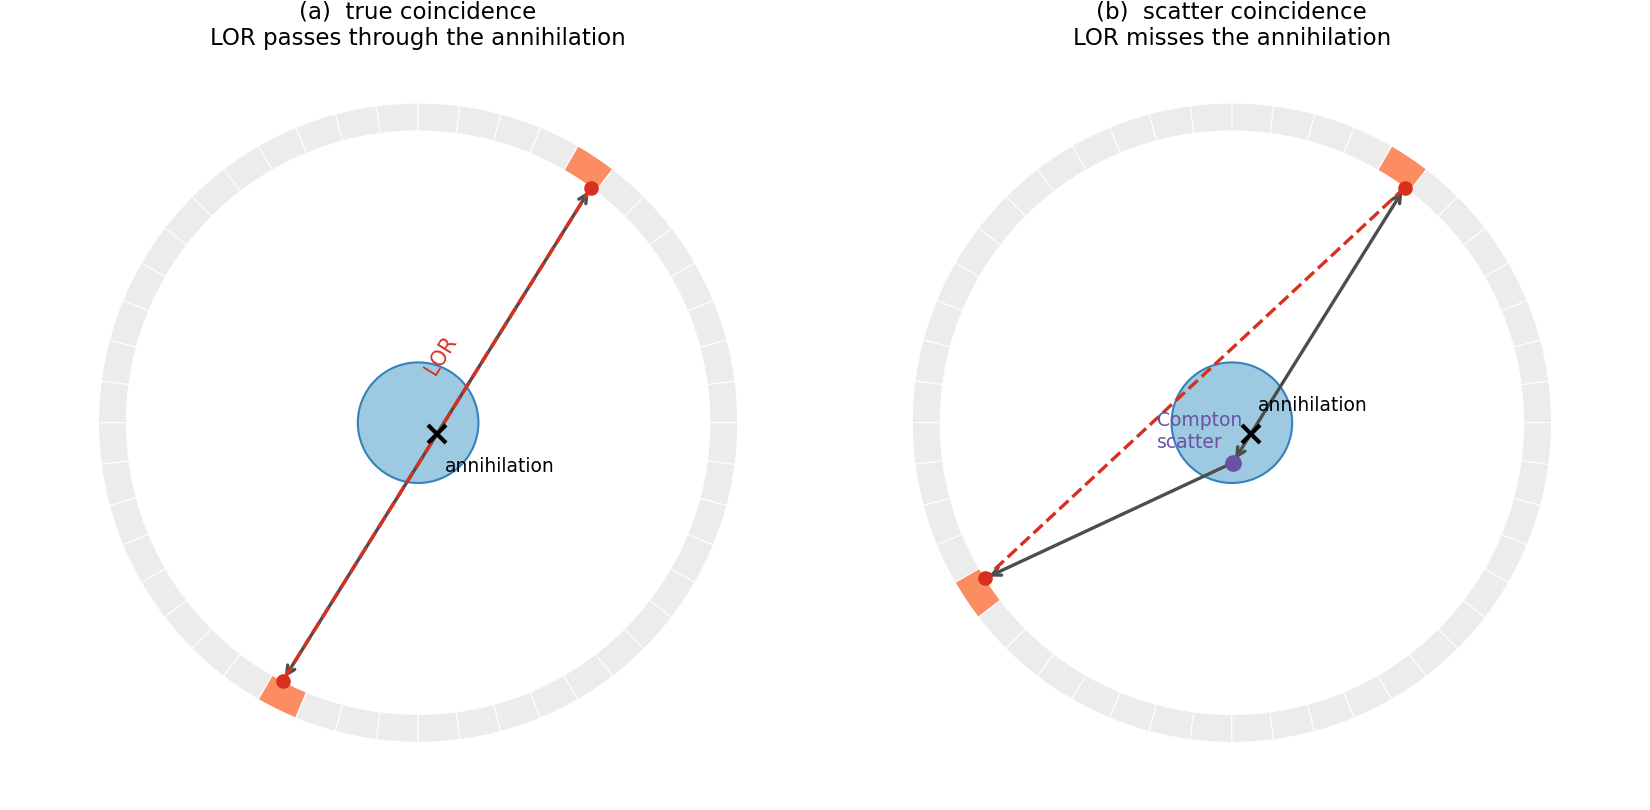
\includegraphics[width=\textwidth]{lor}
  \caption{A coincidence and its line of response. (a) True coincidence: both photons reach the ring
  unscattered and the LOR passes through the annihilation ($\times$). (b) Scatter coincidence: one
  photon Compton-scatters in the phantom, so the LOR between the two hits misses the annihilation.}
  \label{fig:lor}
\end{figure}

\section{Detector response}
\label{sec:detector}

A true hit --- an exact position, a summed energy, an arrival time --- is turned into a measurement
by the detector model.

\subsection{Position and energy resolution}

The position is blurred by an isotropic Gaussian of width $\sigma_{xyz}$, which folds in the
depth-of-interaction uncertainty. The deposited energy is blurred by a resolution that scales as
the square root of the energy,
\begin{equation}
  \mathrm{FWHM}(E) = a\,\sqrt{\SI{511}{keV}\cdot E},
\end{equation}
so the \emph{fractional} resolution is $a\sqrt{\SI{511}{keV}/E}$ and equals $a$ at the photopeak.
The parameter $a$ is the fractional FWHM at \SI{511}{keV} --- the headline number that distinguishes
the crystals.

\subsection{The timestamp: a physical first-photon model}

The arrival time is not a free Gaussian parameter; it follows from the scintillation. A deposit of
energy $E$ produces $N_{\mathrm{det}} = Y\,E\,\mathrm{PDE}$ detected scintillation photons, where
$Y$ is the light yield and PDE the photon-detection efficiency. Each scintillation photon is emitted
after the deposit with a delay drawn from the crystal's decay mixture, whose initial rate is
$r_0 = \sum_k w_k/\tau_k$ over the decay components $(\tau_k, w_k)$. The timestamp is the arrival of
the \emph{first} detected photon --- the minimum of $N_{\mathrm{det}}$ such delays --- so in the
early-time limit
\begin{equation}
  t_{\mathrm{jitter}} = -\,\frac{\ln u}{N_{\mathrm{det}}\,r_0}, \qquad u\sim\mathcal{U}(0,1),
\end{equation}
with mean $1/(N_{\mathrm{det}}\,r_0)$. A bright, fast crystal (large $N_{\mathrm{det}}\,r_0$) times
to a fraction of a nanosecond; a dimmer one is correspondingly slower. The full timestamp adds the
time of flight from the annihilation to the interaction point. This jitter falls out of the
crystal's own light yield, decay, and efficiency, with no tunable $\sigma_t$.

\subsection{Per-crystal properties}

Every quantity above is a property of the crystal and is stored with it in the materials database:
the cross sections, the light yield, the scintillation decay (one or two components, with weights),
the energy resolution $a$, and the PDE. Naming a crystal pulls all of them, so a run is specified by
the crystal name alone. Table~\ref{tab:crystals} lists the monolithic configurations currently
modelled.

\begin{table}[h]
  \centering
  \begin{tabular}{lcccc}
    \hline
    crystal & $a$ (FWHM @ \SI{511}{keV}) & light yield [\si{\gamma/MeV}] & decay [\si{ns}] & $\sigma_{xyz}$ \\
    \hline
    CsI (pure, cryogenic)    & 5\%  & $1.0\times10^{5}$ & 1000            & $\sim\SI{1.7}{mm}$ \\
    BGO (cryogenic)          & 10\% & $2.9\times10^{4}$ & 747 / 2253      & $\sim\SI{1.7}{mm}$ \\
    \hline
  \end{tabular}
  \caption{Monolithic crystals with continuous three-dimensional readout (CRYSP family). The
  position resolution $\sigma_{xyz}$ includes the DOI. The photon-detection efficiency depends on
  the crystal's emission spectrum and is carried per crystal.}
  \label{tab:crystals}
\end{table}

\section*{Reference material}
\addcontentsline{toc}{section}{Reference material}
The CRYSP detector numbers follow Soleti \textit{et al.} (2024). The companion document
\texttt{PTCryspMC\_app} describes the two application modes that drive this engine.

\end{document}
